\documentclass[aspectratio=169]{beamer}
% \documentclass[aspectratio=169, handout]{beamer}
% Add handout option to ignore pauses

% From Jeff E
\usepackage{algo}
\usepackage{sigmastyle}

\usepackage{tabularx}
\newcolumntype{L}{>{\raggedright\arraybackslash}X}

\setbeamertemplate{blocks}[rounded]
\setbeamercovered{transparent}
\usecolortheme{orchid}
\usetheme{sigma}

\graphicspath{{images/}}

\title{Linear time computation for Minimum Spanning Trees}

\author{Ian Chen}
\date{}

% \institute{University of Illinois Urbana-Champaign}

% --------------------------------------------------------------------

% Begin document
\begin{document}

\begin{frame}
    \titlepage
\end{frame}

\section{Preliminaries}

\begin{frame}{Problem Statement}
    \begin{itemize}
        \item Input: $G = (V, E)$, undirected graph with distinct weights.
        \item Output: $T \subset G$ spanning tree minimizing the sum of all edge weights
    \end{itemize}
\end{frame}

\begin{frame}{Heavy and light edges (1/2)}
    \begin{itemize}
        \item An edge is \emph{light} if it is the minimum weight edge across some bipartition
        \item An edge is \emph{heavy} if it is the heaviest weight edge in a cycle
    \end{itemize}

    \only<2>{
        How are these related to minimum spanning trees?
    }
\end{frame}

\begin{frame}{Heavy and light edges (2/2)}
    \begin{table}
        \begin{tabularx}{\linewidth}{| L | L | L | }
            \hline
            Algorithm                    & Light                                       & Heavy                             \\
            \hline
            Kruskals                     & Globally light edge not making cycle        & Adding an edge forms a cycle      \\
            \hline
            Prims                        & Lightest edge crossing frontier             &                                   \\
            \hline
            Boruvkas                     & Lightest edge on partition boundaries       &                                   \\
            \hline
            Chazelle                     & Approximate lightest edge crossing frontier & Adding an edge forms cycle        \\
            \hline
            \textbf{Karger-Klein-Tarjan} & Lightest edges on partition boundaries      & Detect heavy edges wrt a subgraph \\
            \hline
        \end{tabularx}
        \caption{Heavy and light edge classification for selected MST algorithms}
    \end{table}
\end{frame}

\frame{\tableofcontents}

\section{Verifying an MST}
\frame{\tableofcontents[currentsection]}

\begin{frame}{MST Verification}
    \begin{theorem}
        Let $T$ be a spanning tree of $G$.
        $T$ is the (unique) MST if and only if for all edges $uv \in G$
        \begin{equation}
            w(uv) \ge \norm{ \pi^{T}_{uv} }_\infty
            \label{eq:eq1}
        \end{equation}

        where $\pi^{T}_{uv}$ is the unique path betwen $u$ and $v$ in $T$, and $\norm{\cdot}_{\infty}$ is the heaviest edge in the subgraph.
    \end{theorem}
\end{frame}

\begin{frame}{MST Verification}
    \begin{itemize}
        \item How do we check whether Equation \ref{eq:eq1} holds?
              \only<2->{
                  \begin{itemize}
                      \item Reduce the problem to a full-branching tree
                      \item Binary search and clever dynamic programming
                  \end{itemize}
              }
    \end{itemize}
\end{frame}

\begin{frame}{Boruvka Trees}
    \only<1>{
        \begin{itemize}
            \item Vertices in level $i$ of the Boruvka tree is the partition of $G$ after $i$ Boruvka steps
            \item Edges are between adjacent levels whoose vertices are not disjoint (take the heaviest edge)
        \end{itemize}
    }
    \only<2>{
        \begin{figure}
            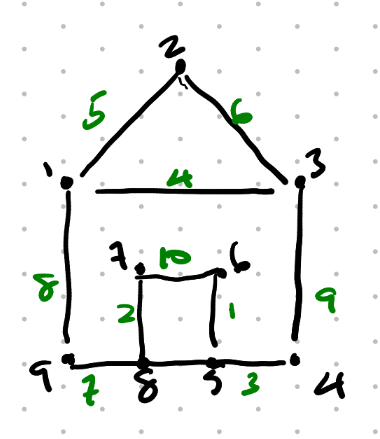
\includegraphics[width=0.3\textwidth]{s1.png}
            \caption{
                Example of Boruvka Tree construction (a), the input graph
            }
        \end{figure}
    }
    \only<3>{
        \begin{figure}
            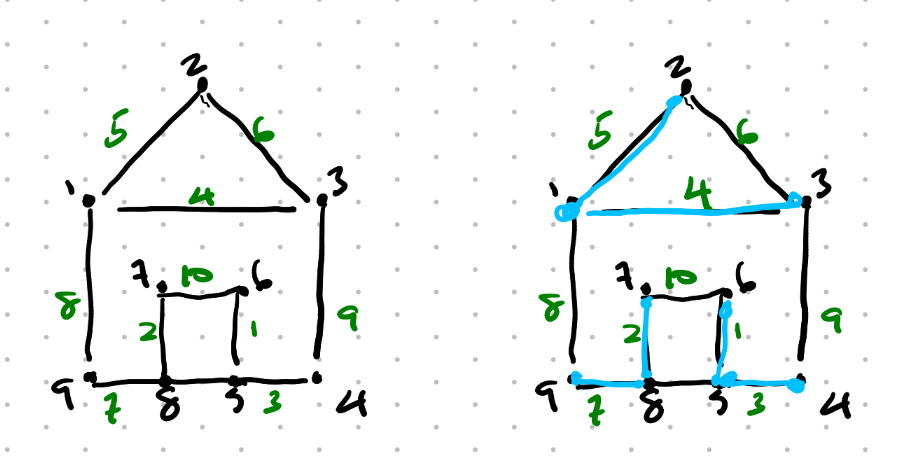
\includegraphics[width=0.8\textwidth]{s2.png}
            \caption{
                Example of Boruvka Tree construction (b), one step of Boruvka
            }
        \end{figure}
    }
    \only<4>{
        \begin{figure}
            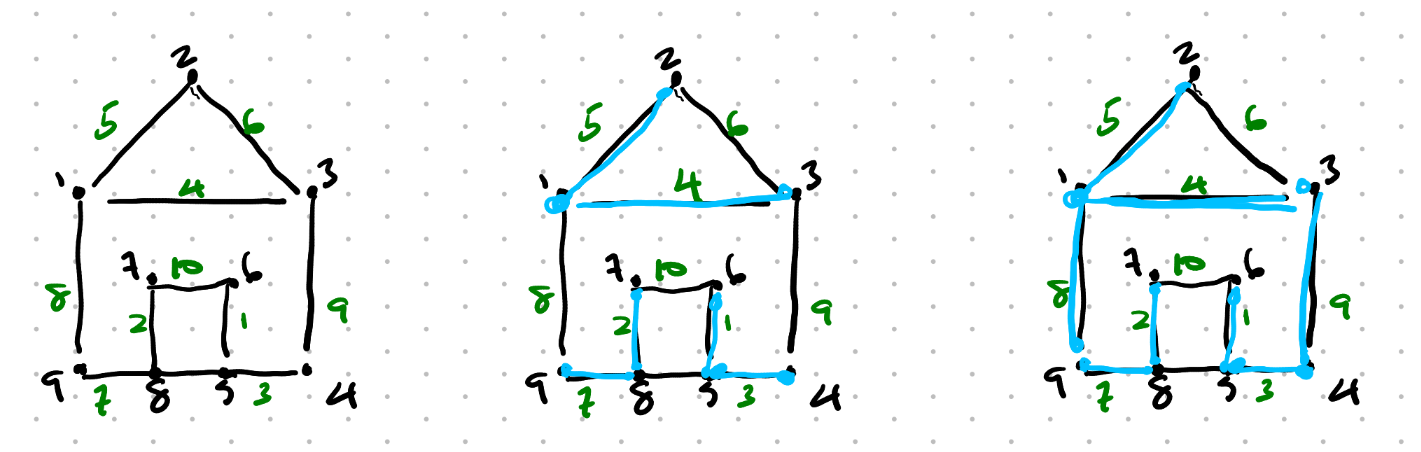
\includegraphics[width=1.0\textwidth]{s3.png}
            \caption{
                Example of Boruvka Tree construction (c), two step of Boruvka.
                Boruvka finds the minimum spanning tree.
            }
        \end{figure}
    }
    \only<5>{
        \begin{figure}
            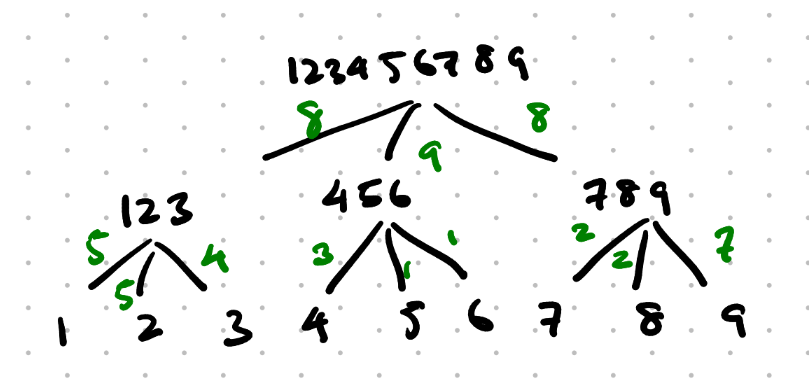
\includegraphics[width=0.8\textwidth]{s4.png}
            \caption{
                Example of Boruvka Tree construction (d), the witness tree.
            }
        \end{figure}
    }
    \only<6>{
        \begin{itemize}
            \item All internal nodes have $\ge 2$ children
            \item All leaves are at same depth
            \item $\norm{\pi^{T}_{uv}}_\infty = \norm{\pi^{B}_{uv}}_\infty$
        \end{itemize}
    }
\end{frame}

\begin{frame}{Querying the Boruvka Tree}
    \begin{itemize}
        \item We have $m$ queries (one for each edge in $G$)
              \pause
        \item Denote $\pi^{B}_{ij} \eval_v$ be the path $\pi^{B}_{ij}$ restricted to $v \rightsquigarrow B.\emph{root}$.
              \pause
        \item Let $f_v: (i, j) \mapsto \norm{\pi^{B}_{ij} \eval_v}_\infty$ for all $(i, j)$ query.
              \pause
        \item $f_v$ is updated from $f_{v.\emph{parent}}$
              \pause
              \begin{itemize}
                  \item Need to update all paths with weight less than $w(v, v.\emph{parent})$
                  \item Keep $f_v$ sorted, binary search to determine which paths update!
              \end{itemize}
    \end{itemize}
\end{frame}

\begin{frame}{Analysis of MST Verification}
    \begin{itemize}
        \item Number of comparisons is bounded by $\sum_v \log( \abs{f_v} + 1 )$
              \pause
        \item $L_i$ vertices on level $i$, $\ell_i = \abs{L_i}$, so $f_v$ are disjoint for $v \in L_i$
              \pause
        \item The log function is convex, so apply Jensen's inequality
              $$
                  \sum_{v \in L_i} \log( \abs{f_v} + 1 ) \le \ell_i \log \left( 1 + \frac{1}{\ell_i} \sum_{v \in L_i} \abs{f_v} \right) \le \ell_i \log \left( 1 + \frac{m}{\ell_i} \right)
              $$
              \pause
              \vspace{-\baselineskip}
        \item Summing over all levels,
              $$
                  \sum_{i} \ell_i \log \left( 1 + \frac{m}{\ell_i} \right) \le 3n + n \log\left( 1 + \frac{m}{n} \right) \le 4n + m
              $$
    \end{itemize}

\end{frame}


\section{Finding an MST}
\frame{\tableofcontents[currentsection]}

\begin{frame}{Strategy}
    \only<1-2>{
        \begin{itemize}
            \onslide<+->
            \item Sufficient to find a linear time algorithm that reduces the number of edges/nodes by constant factor.
                  \onslide<+->
            \item To reduce the number of nodes, can run Boruvka iterations
            \item To reduce the number of edges, (???)
        \end{itemize}
    }
    \only<3->{
        \begin{itemize}
            \item If $e$ is heavy in a $H \subset G$, then $e$ is heavy in $G$.
            \item We say $e$ is $H$-heavy if $e$ is heavy in $H + e$ (otherwise, $e$ is $H$-light).
            \item What subgraph is easy to detect $H$-heavy edges?
        \end{itemize}
    }
\end{frame}

\begin{frame}{Sampling lemma}
    \only<1>{
        \begin{lemma}
            Let $H$ be constructed by picking each edge from $G$ with probability $1/2$.
            Let $F$ be the minimum spanning \emph{forest} of $H$.
            Then, in expectation, $G$ has at most $2n$ $F$-light edges.
        \end{lemma}
    }

    \only<2->{
        \begin{proof}
            \begin{itemize}
                \pause
                \item
                      Label the edges $e_i$ by increasing weight, and let $H_i$ be the subgraph $H \cap \set{e_j \eval j \le i}$ and $F_i$ be the MSF of $H_i$.
                      \pause
                \item
                      If $e_i$ is $F$-light, then $e_i = F_i \setminus F_{i-1}$ with probability $1/2$.
                      \pause
                \item
                      The number of edges in $F$ is less than $n$
                      \pause
                \item
                      Therefore, in expectation $G$ has at most $2n$ $F$-light edges.
            \end{itemize}
        \end{proof}
    }
\end{frame}

\begin{frame}{KKT algorithm}
    \begin{enumerate}
        \item If $\abs{G} = 1$, uncontract any components and return the MST.
        \item $G' \gets G$ after $2$ Boruvka iterations
        \item Subsample a graph $H \subset G'$ with probability $1/2$
        \item Find the MSF $F$ of $H$
        \item $G \gets G'$ after removing all $F$-heavy edges
        \item Goto step 1
    \end{enumerate}
\end{frame}

\begin{frame}{Analysis}
    \begin{theorem}
        Let $T(n, m)$ be the runtime of the KKT algorithm.
        Then, $\mathbf{E}(T(n, m)) = O(n+m)$.
    \end{theorem}

    \begin{proof}
        \only<1>{
            $$
                T(n, m) = T(n/4, \tilde{m}_1) + T(n/4, \tilde{m}_2) + O(n+m)
            $$
            where $\tilde{m}_1 = \abs{E(H)}$, $\tilde{m}_2$ is the number of $F$-light edges.
            Observe that $\mathbf{E}(\tilde{m}_1) = m/2$ and $\textbf{E}(\tilde{m}_2) \le 2 \cdot n/4 = n/2$.
        }

        \only<2>{
            Supposing that $\mathbf{E}(T(n', m'))$ is linear from $n' < n$ and $m' < m$, then
            \begin{align*}
                \mathbf{E}(T(n,m)) & = \mathbf{E}(T(n/4, \tilde{m}_1)) + \mathbf{E}(T(n/4, \tilde{m}_2)) + O(n+m)                         \\
                                   & = \mathbf{E}(T(n/4, \mathbf{E}(\tilde{m}_1))) + \mathbf{E}(T(n/4, \mathbf{E}(\tilde{m}_2))) + O(n+m) \\
                                   & = \mathbf{E}(T(n/4, m/2)) + \mathbf{E}(T(n/4, n/2)) + O(n+m)                                         \\
                                   & = O(n+m)
            \end{align*}
        }
    \end{proof}
\end{frame}

\begin{frame}[allowframebreaks]{Bibliography}
    \bibliographystyle{alpha}
    \begin{itemize}
        \item David R. Karger, Philip N. Klein, and Robert E. Tarjan. 1995. A randomized linear-time algorithm to find minimum spanning trees. J. ACM 42, 2 (March 1995), 321–328. \url{https://doi.org/10.1145/201019.201022}
        \item Komlós, J. Linear verification for spanning trees. Combinatorica 5, 57–65 (1985). \url{https://doi.org/10.1007/BF02579443}
        \item King, V. (1995). A simpler minimum spanning tree verification algorithm. In: Akl, S.G., Dehne, F., Sack, JR., Santoro, N. (eds) Algorithms and Data Structures. WADS 1995. Lecture Notes in Computer Science, vol 955. Springer, Berlin, Heidelberg. \url{https://doi.org/10.1007/3-540-60220-8_83}
    \end{itemize}
\end{frame}



\end{document}
